\subsection{Autenticação Baseada em Token}

\emph{Tokens} são itens utilizados para identificar e autenticar usuários. São palavras assinadas e 
não criptografadas, que carregam informações sobre um usuário autenticado \cite{BALAJ2017}. O 
padrão mais utilizado deste tipo de autenticação é o JSON \emph{Web Token} (JWT), que foi proposto
na RFC 7519. O JWT é um formato compacto de representação de reinvindicações (\emph{claims}), 
destinado a ambientes com restrição de espaço, como cabeçalhos HTTP e parâmetros de consulta de URI 
\cite{RFC7519}.

Um JSON Web Token é composto por cadeias de caracteres codificadas em base64url, separadas 
por ponto. Geralmente possuem 3 cadeias: o cabeçalho, que contém informações a respeito do tipo de mídia do 
JWT e da criptografia usada para assinar o \emph{token}; a carga útil (\emph{payload}), que contém 
as informações sobre as \emph{claims}, que são conjuntos de declarações sobre uma entidade 
(geralmente um usuário); e a assinatura, que é a concatenação dos \emph{hashes} gerados a partir das 
outras duas cadeias com uma chave secreta ou certificado, utilizada para verificação de integridade
do \emph{token} \cite{MONTANHEIRO2017}.

Neste método, após o envio de credenciais de acesso e validação do usuário por meio de uma 
requisição HTTP, o servidor gera um \emph{token}, que é enviado para o cliente e pode ser salvo
em \emph{cookies} ou no armazenamento local \cite{MONTANHEIRO2017}. Também pode ser enviado um 
\emph{token} de atualização (\emph{refresh token}), para a obtenção de um novo \emph{token} de acesso
assim que o atual expirar. Ao possuir o \emph{token}, quando uma requisição é feita ao servidor o 
mesmo deve ser enviado no cabeçalho \texttt{Authorization}, precedido pela palavra \emph{Bearer}. 
\cite{RFC6749}. (Figura \ref{fig:tokenAuth})

\begin{figure}[ht]
    \centering
    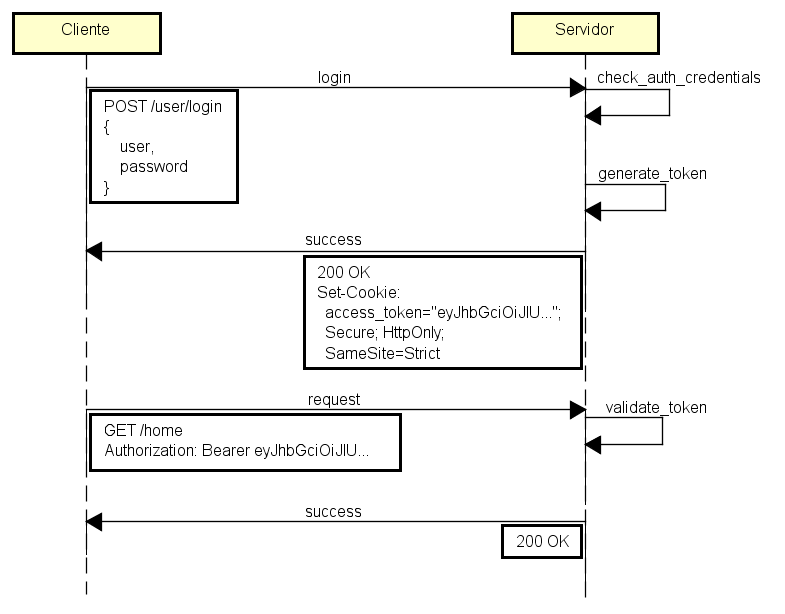
\includegraphics[width=.8\textwidth]{Token-Based Authentication.png}
    \caption{Exemplo de Autenticação baseada em \emph{token}}
    \label{fig:tokenAuth}
  \end{figure}